%%%%%%%%%%%%%%%%%%%%%%%%%%%%%%%%%%%%%%%%%%%
%%%%%%%%%%%%%%%%%%%%%%%%%%%%%%%%%%%%%%%%%%%
%%%%%%%%%%%%%%% CHAPTER 14 %%%%%%%%%%%%%%%%


\section{Modelagem: sistemas eletromecânicos}

\frame{
\frametitle{Introdução}
\begin{block}{Sistemas híbridos}
Diversos equipamentos e componentes podem ser construídos ao se combinar varáveis \textbf{elétricas} e \textbf{mecânicas}, formando os \textbf{sistemas eletromecânicos}.
\end{block}
}

\frame{
\frametitle{Introdução}
\begin{block}{Aplicações}
\begin{itemize}
    \item Sistema de controle de posição de azimute de antena
    \item Controle de robôs
    \item Potenciômetros
    \item Galvanômetros
    \item Microfones
    \item Motores e geradores
\end{itemize}
\end{block}
}

\frame{
\frametitle{Introdução}
\begin{block}{Acoplamento}
O acoplamento de sistemas eletromecânicos pode ser dado de duas formas:
\begin{enumerate}
    \item Acoplamento \textbf{resistivo}
    \item Acoplamento por \textbf{campo magnético}
\end{enumerate}
\end{block}
}

\frame{
\frametitle{Acoplamento resistivo}
\begin{block}{Introdução}
É possível controlar uma \textbf{resistência variável} por meio de movimentos \textbf{mecânicos} ao mover continuamente um contato \textbf{elétrico}.
\begin{itemize}
    \item Este método de acoplamento não envolve forças mecânicas que dependem de varáveis elétricas, visto que resistores não podem armazenar energia.
\end{itemize}
\end{block}
}

\frame{
\frametitle{Acoplamento resistivo}
\begin{block}{Resistores variáveis}
Considere uma barra de um material condutor com resistividade $\rho$ e área da seção transversal $A$.
\begin{itemize}
    \item Um terminal é fixo e o outro está livre para se movimentar.
    \item A resistência por unidade de área é dada por $\rho/A$.
\end{itemize}
$$\boxed{R = \dfrac{\rho}{A} x(t)}$$
\end{block}
\vspace{0.3cm}
\centerline{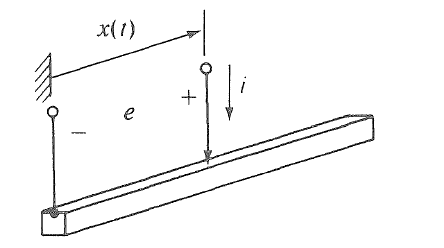
\includegraphics[width=0.5\linewidth]{Figuras/Ch14/fig1.PNG}}
}

\frame{
\frametitle{Acoplamento resistivo}
\begin{block}{Potenciômetro}
Um \textbf{potenciômetro} é um dispositivo onde um \textbf{terceiro} terminal é adicionado no esquema do resistor variável.
\begin{itemize}
    \item A tensão no terminal móvel é considerada a saída do sistema ($e_0$).
    \item As resistências $R_1$ e $R_2$ dependem da posição do terminal central (móvel).
\end{itemize}
\end{block}
\vspace{0.3cm}
\centerline{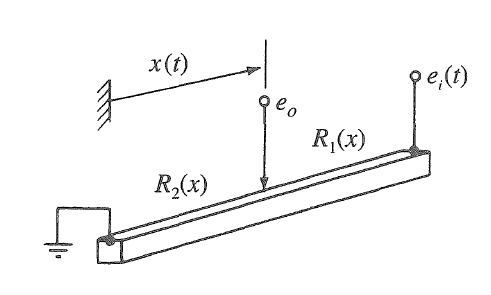
\includegraphics[width=0.5\linewidth]{Figuras/Ch14/fig2.PNG}}
}

\frame{
\frametitle{Acoplamento resistivo}
\begin{block}{Potenciômetro}
O \textbf{circuito elétrico} equivalente, considerando que os dois terminais fixos estão conectados à uma fonte de tensão pode ser visto a seguir.
\begin{itemize}
    \item Utilizando o \textbf{divisor de tensão}, temos:
\end{itemize}
$$\boxed{e_0 = \left(\dfrac{R_2}{R_1+R_2}\right) e_i(t)}$$
\end{block}
\vspace{0.3cm}
\centerline{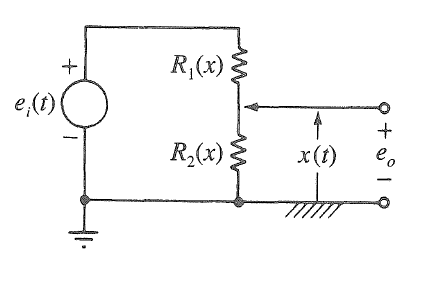
\includegraphics[width=0.5\linewidth]{Figuras/Ch14/fig3.PNG}}
}

\frame{
\frametitle{Acoplamento resistivo}
\begin{block}{Potenciômetro}
\begin{itemize}
    \item Distância entre os terminais fixos (comprimento total): $x_{max}$
    \item Resistência entre os terminais fixos (resistência total): $R_T$
\end{itemize}
$$R_2 = \dfrac{R_T}{x_{max}} x(t) \qquad R_T = R_1 + R_2$$
Logo,
$$\boxed{e_0 = \dfrac{x(t)}{x_{max}} e_i(t)}$$

onde $0 \leq \dfrac{x(t)}{x_{max}} \leq 1$

\begin{itemize}
    \item A \textbf{tensão de saída} ($e_0$) é proporcional ao produto da \textbf{tensão de entrada} ($e_i(t)$) e a variável \textbf{mecânica} ($x(t)$).
\end{itemize}
\end{block}
}

\frame{
\frametitle{Acoplamento resistivo}
\begin{block}{Potenciômetro rotativo}
$$\boxed{e_0 = \dfrac{\theta(t)}{\theta_{max}} E}$$
\end{block}
\vspace{0.1cm}
\centerline{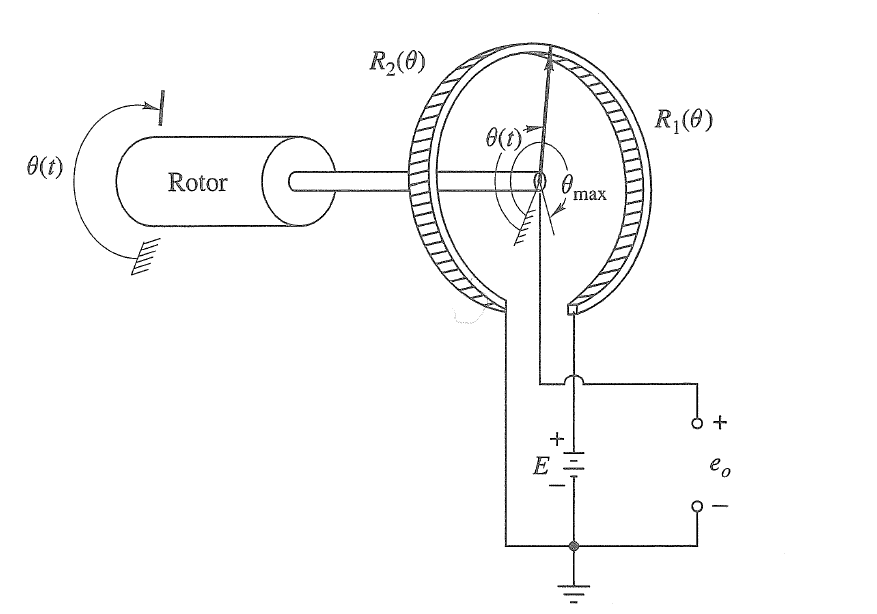
\includegraphics[width=0.65\linewidth]{Figuras/Ch14/fig4.PNG}}
}

\frame{
\frametitle{Acoplamento resistivo}
\begin{block}{Efeito de carga}
\begin{itemize}
    \item A saída de um potenciômetro é frequentemente conectado a algum componente elétrico (\textbf{carga}).
    \item Este efeito de carga pode ser modelado por um resistor externo $R_0$, conectado à \textbf{saída do potenciômetro}.
\end{itemize}
\end{block}
\vspace{0.1cm}
\centerline{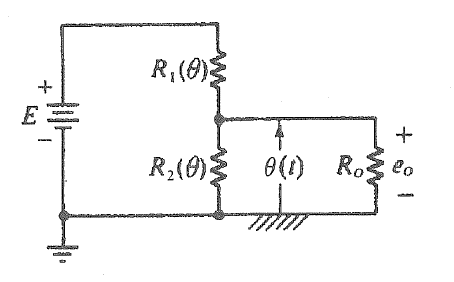
\includegraphics[width=0.5\linewidth]{Figuras/Ch14/fig5.PNG}}
}

\frame{
\frametitle{Acoplamento resistivo}
\begin{block}{Efeito de carga}
\begin{itemize}
    \item Não é possível mais utilizar a fórmula de divisor de tensão pois $R_1$ e $R_2$ não estão mais em série.
    \item Consequentemente, a relação de $e_0$ com o deslocamento mecânico (translacional ou rotacional) também \textbf{não é mais válido}.
    \item Para contornar este problema, pode-se fazer $R_0$ \textbf{muito maior} se comparado com $R_2$. Como $R_2 \leq R_T$, temos:
    $$R_0 \gg R_T$$
    \item Com isso, a corrente em $R_0$ é \textbf{negligenciável}, e $R_1$ estará em \textbf{série} com $R_2$ (efeito de carga foi desprezado).
\end{itemize}
\end{block}
}

\frame{
\frametitle{Acoplamento por campo magnético}
\begin{block}{Introdução}
Uma grande variedade de dispositivos eletromecânicos envolve o \textbf{fluxo de corrente elétrica} dentro de um \textbf{campo magnético}.
\end{block}
}

\frame{
\frametitle{Acoplamento por campo magnético}
\begin{block}{Princípios}
\begin{enumerate}
    \item Um condutor percorrido por corrente elétrica quando imerso em um campo magnético sofre a ação de uma \textbf{força eletromagnética}.
    \item Uma \textbf{tensão} será induzida num condutor quando este se move relativamente à um campo magnético.
\end{enumerate}
\end{block}
}

\frame{
\frametitle{Acoplamento por campo magnético}
\begin{block}{Força eletromagnética}
A força eletromagnética ($f_e$) é dada pela equação abaixo:
$$\boxed{f_e = \euscr{B} \cdot \ell \cdot i \cdot \text{sen}\gamma}$$
onde 
\begin{itemize}
    \item $\euscr{B}$ é a densidade de fluxo magnético
    \item $\ell$ é o comprimento do condutor sob o efeito do campo magnético
    \item $i$ é a corrente elétrica que percorre o condutor
    \item $\gamma$ é o ângulo entre as linhas de campo e a superfície longitudinal do condutor
\end{itemize}
\end{block}
}

\frame{
\frametitle{Acoplamento por campo magnético}
\begin{block}{Força eletromagnética}
Considerando que o condutor seja perpendicular ao campo magnético, temos:
$$\gamma = \SI{90}{\degree} \implies \text{sen}\gamma = 1$$
Com isso,
$$\boxed{f_e = \euscr{B} \cdot \ell \cdot i}$$
onde a \textbf{direção} de $f_e$ é sempre \textbf{perpendicular} ao condutor e também ao campo magnético.
\end{block}
}

\frame{
\frametitle{Acoplamento por campo magnético}
\begin{block}{Força eletromagnética}
A regra da mão esquerda, chamada de “regra da mão esquerda de Fleming”, é usada para encontrar o \textbf{sentido da força eletromagnética}.
\begin{itemize}
    \item O dedo \textbf{polegar} representa o sentido da força eletromagnética ($f_e$).
    \item Já o dedo \textbf{indicador} representa o sentido do fluxo magnético ($\euscr{B}$).
    \item O dedo \textbf{médio} indica o sentido da corrente elétrica ($i$).
\end{itemize}
\end{block}
\centerline{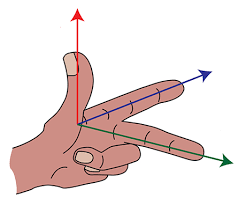
\includegraphics[width=0.45\linewidth]{Figuras/Ch14/fig6.PNG}}
}

\frame{
\frametitle{Acoplamento por campo magnético}
\begin{block}{Tensão induzida}
A lei de Faraday enuncia que em todo condutor, enquanto sujeito a uma variação de fluxo magnético, é estabelecida uma \textbf{força eletromotriz} (tensão) induzida. Esta força eletromotriz ($e_m$) é dada pela equação abaixo:
$$\boxed{e_m = \euscr{B} \cdot \ell \cdot v \cdot \text{sen}\gamma}$$
onde 
\begin{itemize}
    \item $\euscr{B}$ é a densidade de fluxo magnético
    \item $\ell$ é o comprimento do condutor sob o efeito do campo magnético
    \item $v$ é a velocidade do condutor no campo magnético
    \item $\gamma$ é o ângulo de deslocamento do condutor em relação as linhas de campo
\end{itemize}
\end{block}
}

\frame{
\frametitle{Acoplamento por campo magnético}
\begin{block}{Tensão induzida}
Considerando que o condutor seja perpendicular ao campo magnético, temos:
$$\gamma = \SI{90}{\degree} \implies \text{sen}\gamma = 1$$
Com isso,
$$\boxed{e_m = \euscr{B} \cdot \ell \cdot v}$$
onde a \textbf{direção} de $e_m$ é sempre \textbf{perpendicular} ao condutor e também ao campo magnético.
\end{block}
}

\frame{
\frametitle{Exemplo $\#01$ - galvanômetro}
\begin{block}{}
O \textbf{galvanômetro} é um equipamento que produz uma \textbf{deflexão angular} dependendo da \textbf{corrente} que passa nele.
\end{block}
\centerline{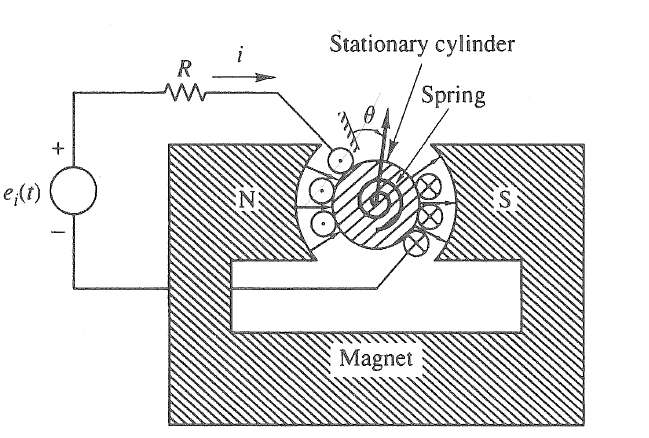
\includegraphics[width=0.7\linewidth]{Figuras/Ch14/fig7.PNG}}
}

\frame{
\frametitle{Exemplo $\#01$ - galvanômetro}
\begin{block}{Princípio de funcionamento}
\begin{itemize}
    \item Um \textbf{ímã} permanente fornece o campo magnético e o fluxo magnético passa através de um núcleo estacionário (localizado entre os polos do ímã).
    \item Uma \textbf{bobina} cujos terminais são conectados a um \textbf{circuito externo} é suspensa por um rolamento/mancal, permitindo a rotação ao longo do eixo horizontal.
    \item A corrente flui \textbf{para fora} da página no lado esquerdo e \textbf{para dentro} da página no lado direito.
\end{itemize}
\end{block}
}

\frame{
\frametitle{Exemplo $\#01$ - galvanômetro}
\begin{block}{Princípio de funcionamento}
\begin{itemize}
    \item O ímã produz uma densidade de fluxo magnético constante $\euscr{B}$.
    \item O momento de inércia da bobina é $J$.
    \item O atrito do rolamento/mancal é representado por $B$.
    \item A mola torcional possui constante $K$.
\end{itemize}
\end{block}
\vspace{0.2cm}
\centerline{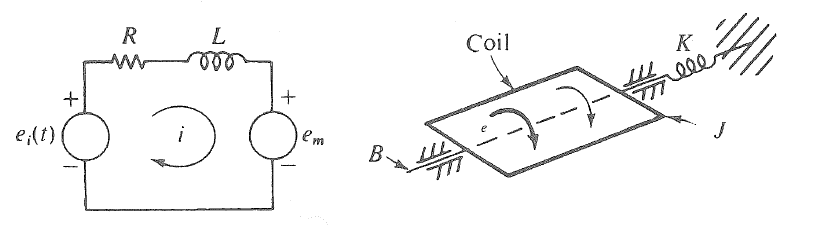
\includegraphics[width=0.9\linewidth]{Figuras/Ch14/fig8.PNG}}
}

\frame{
\frametitle{Exemplo $\#01$ - galvanômetro}
\begin{block}{Princípio de funcionamento}
\begin{itemize}
    \item A bobina consiste de $N$ voltas retangulares, cada uma com raio $a$ e comprimento $\ell$ ao longo da direção do eixo de rotação.
    \item A indutância total da bobina é $L$.
    \item A fonte de tensão externa é $e_i(t)$.
    \item A resistência $R$ modela toda resistência externa do galvanômetro, além da resistência das bobinas.
\end{itemize}
\end{block}
\vspace{0.2cm}
\centerline{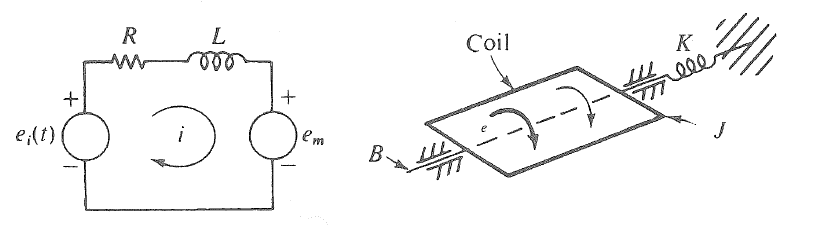
\includegraphics[width=0.9\linewidth]{Figuras/Ch14/fig8.PNG}}
}

\frame{
\frametitle{Exemplo $\#01$ - galvanômetro}
\begin{block}{Formulação matemática}
\begin{itemize}
    \item O \textbf{torque} ($\tau_e$) agindo sobre o eixo da bobina é dado pela soma de torques dos $2N$ condutores individuais de comprimento $\ell$.
    \item Cada condutor do lado esquerdo da bobina possui uma \textbf{força} $f_e = \euscr{B} \cdot \ell \cdot i$ agindo para cima; ao passo que cada condutor do lado direito da bobina possui uma força de mesma intensidade agindo para baixo.
\end{itemize}
Deste modo,
$$\tau_e = 2N \euscr{B} \ell a i$$
Além disso, existem $2N$ condutores em série que se movem a uma velocidade $a\dot{\theta}$ em relação ao campo magnético. Com isso,
$$e_m = 2N \euscr{B} \ell a \dot{\theta}$$
\end{block}
}

\frame{
\frametitle{Exemplo $\#01$ - galvanômetro}
\begin{block}{Formulação matemática}
As equações que modelam este sistema eletromecânico são, portanto:
\begin{equation*}
\begin{cases}
Ri + L\dfrac{di}{dt} + 2N \euscr{B} \ell a \dot{\theta} = e_i(t) \\
J\ddot{\theta} + B\dot{\theta} + K\theta = 2N \euscr{B} \ell a i
\end{cases}
\end{equation*}
Em situações práticas, a \textbf{indutância na bobina é muito pequena}, permitindo anular o segundo termo da primeira equação. Logo,
$$i = \dfrac{1}{R} \left(e_i(t) - 2N \euscr{B} \ell a \dot{\theta} \right)$$
Substituindo essa nova equação na segunda equação, vem:
$$\ddot{\theta} + \left(\dfrac{B}{J} + \dfrac{\alpha^2}{JR}\right)\dot{\theta} + \dfrac{K}{J}\theta = \dfrac{\alpha}{JR}e_i(t)$$
onde $\alpha = 2N \euscr{B} \ell a$ é o \textbf{coeficiente de acoplamento eletromagnético}.
\end{block}
}

\frame{
\frametitle{Exemplo $\#02$ - microfone}
\begin{block}{}
O \textbf{microfone} consiste de uma diafragma ligado a uma bobina circular que se move para frente e para trás através de um campo magnético quando ondas de som colidem no diafragma.
\end{block}
\vspace{0.4cm}
\centerline{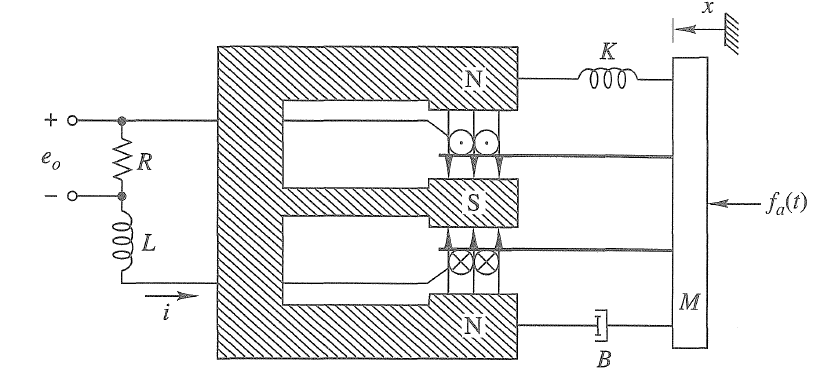
\includegraphics[width=0.8\linewidth]{Figuras/Ch14/fig9.PNG}}
}

\frame{
\frametitle{Exemplo $\#02$ - microfone}
\begin{block}{Princípio de funcionamento}
\begin{itemize}
    \item Um \textbf{ímã} permanente cilíndrico fornece o campo magnético.
    \item A \textbf{bobina} possui $N$ voltas com um raio $a$ e está conectada em série com um resistor externo $R$ (onde a \textbf{tensão de saída} é medida).
    \item A resistência da bobina é negligenciada, mas a sua indutância é representada por $L$.
    \item Um único elemento $K$ é usado para modelar a rigidez do diafragma.
    \item O elemento de atrito viscoso $B$ representa a dissipação de energia devido a resistência do ar.
    \item A força resultante das ondas sonoras incidentes é representada por $f_a(t)$ (\textbf{entrada do sistema}).
\end{itemize}
\end{block}
}

\frame{
\frametitle{Exemplo $\#02$ - microfone}
\begin{block}{Princípio de funcionamento}
\begin{itemize}
    \item A figura abaixo mostra a porção superior de uma simples volta de uma bobina, com uma vista do diafragma para o ímã.
    \item Para determinar o \textbf{sentido positivo} de $f_e$ devemos utilizar a regra da mão esquerda, que neste caso, é em direção ao diafragma.
\end{itemize}
\end{block}
\vspace{0.3cm}
\centerline{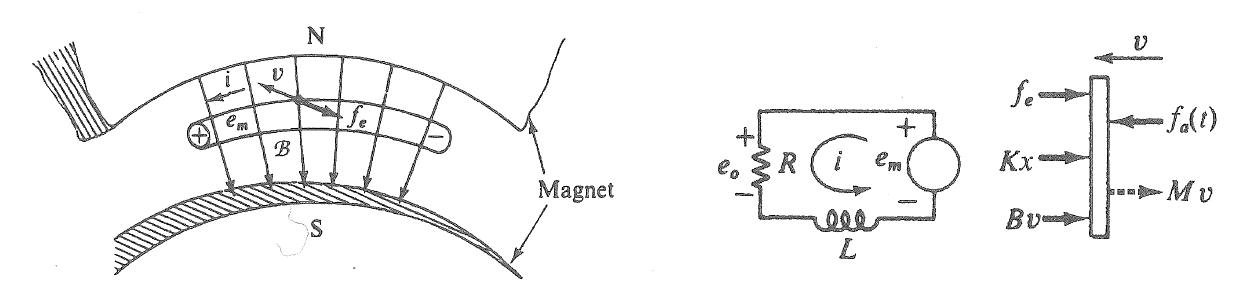
\includegraphics[width=1\linewidth]{Figuras/Ch14/fig10.PNG}}
}

\frame{
\frametitle{Exemplo $\#02$ - microfone}
\begin{block}{Formulação matemática}
\begin{itemize}
    \item O \textbf{comprimento} $\ell$ de toda bobina é dado por $2\pi a N$.
\end{itemize}
Deste modo,
$$f_e = \alpha i$$
$$e_m = \alpha \dot{x}$$
onde $\alpha = 2\pi a N \euscr{B}$ é o \textbf{coeficiente de acoplamento eletromagnético}.

\vspace{0.3cm}

As equações que modelam este sistema eletromecânico são, portanto:
\begin{equation*}
\begin{cases}
M\ddot{x} + B\dot{x} + Kx = -\alpha i + f_a(t)\\
Ri + L\dfrac{di}{dt} = \alpha \dot{x} \\
e_0 = Ri
\end{cases}
\end{equation*}
\end{block}
}

\frame{
\frametitle{Exemplo $\#03$}
\begin{block}{Problema}
Um fio de comprimento $\ell$, rigidamente preso a uma massa $M$, está em um campo magnético com densidade de fluxo $\euscr{B}$. Na vista da seção transversal, o fio é perpendicular à página, com o ponto $a$ conectado à frente do fio e ponto $b$ para trás. A entrada do sistema é uma bateria de 12 Volts. Suponha que não haja energia armazenada inicialmente dentro do sistema e que o interruptor fecha em $t = 0$ s. Qual será o deslocamento em regime permanente da massa a partir de sua posição original?
\end{block}
\centerline{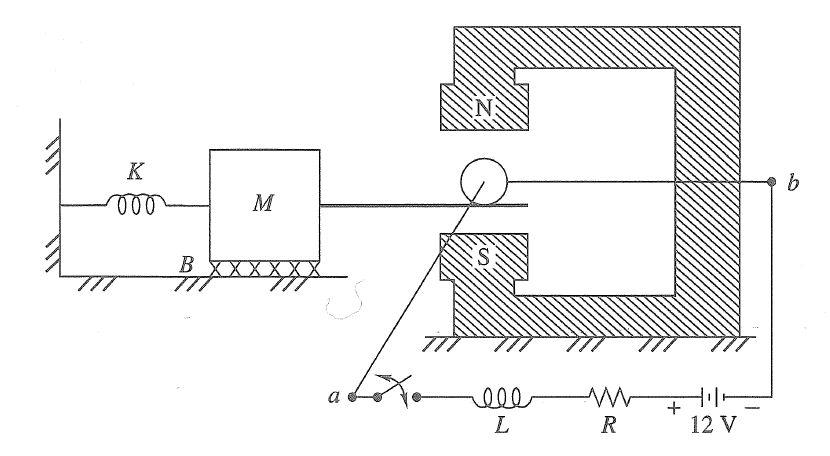
\includegraphics[width=0.6\linewidth]{Figuras/Ch14/fig11.PNG}}
}

\frame{
\frametitle{Exemplo $\#03$}
\begin{block}{Solução}
\begin{itemize}
    \item Utilizando a regra da mão esquerda, temos que $f_e$ está para a esquerda, logo, o deslocamento de $M$ será para a esquerda.
\end{itemize}
\vspace{0.2cm}
As equações que modelam este sistema eletromecânico são, portanto:
\begin{equation*}
\begin{cases}
Ri + L\dfrac{di}{dt} = 12 - \euscr{B} \ell v \\
M\ddot{x} + B\dot{x} + Kx = \euscr{B} \ell i
\end{cases}
\end{equation*}
\end{block}
}

\frame{
\frametitle{Exemplo $\#03$}
\begin{block}{Solução}
Em regime permanente (equilíbrio), com a massa parada, não haverá mais tensão induzida no fio.

\vspace{0.2cm}

Da primeira equação, temos:
$$R i_{ss} + 0 = 12 - 0 \implies i_{ss} = \dfrac{12}{R}$$

Da segunda equação, temos:
$$0 + 0 + K x_{ss} = \euscr{B} \ell i = \euscr{B} \ell \dfrac{12}{R} \implies x_{ss} = \dfrac{12 \euscr{B} \ell}{KR}$$
\end{block}
}

\frame{
\frametitle{Exercícios}
\begin{block}{}
01. Para o exemplo do microfone visto em sala de aula, mostre que:

\vspace{0.2cm}

(a) a função de transferência é dada por
$$H(s) = \dfrac{E_0(s)}{F_a(s)} = \dfrac{\alpha Rs}{MLs^3 + (MR + BL)s^2 + (KL + BR + \alpha^2)s + KR}$$

(b) quando $L=0$, a frequência natural $\omega_n$ e o coeficiente de amortecimento $\zeta$ são dados por
$$\omega_n = \sqrt{\dfrac{K}{M}}$$
$$\zeta = \dfrac{\alpha^2 + BR}{2R\sqrt{MK}}$$
\end{block}
}

\frame{
\frametitle{Referências e exercícios complementares}
\begin{itemize}
\item CLOSE, Charles M.; FREDERICK, Dean K.; NEWELL, Jonathan C. Modeling and Analysis of Dynamic Systems, 3 ed. John Wiley \& Sons, 2003.
\end{itemize}
\centering{\alert{Página 361 - \textbf{Capítulo 10}}} \\
}